\documentclass[conference]{IEEEtran}
\IEEEoverridecommandlockouts

\usepackage{cite}
\usepackage{amsmath,amssymb}
\usepackage{graphicx}
\usepackage{booktabs}
\usepackage{tabularx}
\usepackage{array}
\usepackage{url}
\usepackage{balance}

\title{RecheckLab: When Does Learned Gating Improve LLM Self-Verification?\\
Recorded Replay and Independent Local Inference}

\author{\IEEEauthorblockN{Anonymous Authors}}

\begin{document}
\maketitle

\begin{abstract}
Repeated language-model verification can repair an incorrect answer, leave it unchanged, or damage a correct answer. We compare the frozen RecheckLab v0.2 gate with never-recheck, always-recheck, and completion-based policies, first by replaying SEVRA response records and then on two separately collected local-inference cohorts. The historical replay analysis uses a 19-feature gate and a fixed development-selected threshold; it shows no demonstrated incremental accuracy over completion-based selection. In fresh Qwen3-4B-Instruct-2507 local runs, a 40-question GSM8K sample yielded 37/40 correct initial answers and 38/40 with revision; on a prospectively selected exact-numeric/rational MATH Level 4--5 subset, 43 of 60 frozen questions formed complete pairs before the run was stopped, with 41/43 and 42/43 correct, respectively. In both cohorts, the completion heuristic and the frozen gate selected zero rechecks and therefore matched never-recheck accuracy, missing the single observed helpful revision. All completed responses were parseable; an independent exact regrade matched all 86 MATH call labels and verified the selected reference keys against the pinned benchmark source. The Instruct runs differ from the SEVRA protocol and constitute cross-model/cross-protocol out-of-distribution diagnostics, not deployment validation. The MATH subset is restricted to unambiguous exact answers, and early stopping may induce difficulty- and runtime-related selection bias. These small studies do not establish significance, equivalence, or generalization. The evidence supports the need for prospective, multi-protocol validation with calibrated answer measurement and measured serving costs.
\end{abstract}

\begin{IEEEkeywords}
large language models, self-verification, selective inference, policy evaluation, recorded-response replay, cost-aware inference
\end{IEEEkeywords}

\section{Introduction}
Asking a language model to reconsider an answer is an inference-time intervention with asymmetric outcomes. It may repair an error (HELP), preserve correctness or incorrectness (NO\_CHANGE), or turn a correct response into an incorrect one (HURT). Rechecking every answer incurs the cost of a second model call, including when the answer would not change. A selective policy can reduce this cost, but a learned selector also adds complexity and may not outperform a simple signal such as whether the initial generation exhausted its token budget.

RecheckLab studies whether an initial-response classifier can predict the value of an LLM self-verification step. The active v0.2 model predicts HELP, NO\_CHANGE, and HURT from 19 features available before the recheck. It then maps those probabilities to a binary recheck decision. Earlier project analyses found that the learned gate ties a completion heuristic on CommonsenseQA and does not improve source-test accuracy on MATH. The response records originate from SEVRA, which itself studies selective verification and budget allocation~\cite{dip2026sevra}. Thus, the relevant question is not whether RecheckLab has discovered selective verification, but whether this frozen lightweight classifier adds measurable value over a completion rule when both act on the same recorded attempts.

This paper provides a cross-domain, question-clustered evaluation of four implementable policies and a hindsight-only oracle. The source MATH holdout, CommonsenseQA target partition, MATH500, and GSM8K are kept separate. For the historical cohorts, we reuse saved v0.2 predictions; MATH500 and GSM8K are scored with the unchanged artifact. We separately report new local inference on GSM8K and a selected MATH subset, using saved initial/revision pairs for each policy. We do not retrain or select thresholds on evaluation data. Importantly, the source MATH test set is a question-group holdout from the SEVRA MATH-training split, not a verified official MATH Level 5 evaluation. The additional MATH500 split is a different cohort.

Our contributions are bounded empirical findings:
\begin{itemize}
  \item We report paired policy outcomes and recorded token costs under question-equal weighting, keep repeated rollouts within question clusters, and separate call reduction from revision-token reduction.
  \item We apply the frozen gate to two additional SEVRA evaluation logs, MATH500 and GSM8K, as exploratory external replay diagnostics.
  \item We document a negative result for incremental learning value in historical SEVRA replays and report two independent local-inference cohorts, where the learned and completion gates made no rechecks under a different protocol.
\end{itemize}

The evidence comprises four distinct scopes: (1) historical recorded-response replay on SEVRA source/target cohorts; (2) exploratory replay on SEVRA MATH500 and GSM8K logs; (3) prospective local inference on newly selected GSM8K and MATH questions; and (4) cross-model/cross-protocol OOD application of the frozen gate to those local responses. The local runs do not validate deployed gate behavior. Replayed timings are based on measured individual calls, not end-to-end selective serving.

\section{Related Work}
\subsection{Selective verification and the SEVRA data source}
SEVRA (Selective Verification for Reasoning Allocation) studies when to preserve a frozen solver's initial answer or invoke active verification, using a Qwen3-4B solver, logged intervention outcomes, and recoverability-aware gates~\cite{dip2026sevra}. Its published results also compare verification with longer initial solving, and report harmful revisions and token use. The paired response release used here is derived from this research. RecheckLab is therefore a secondary analysis of these records, not an independent replication of SEVRA's original data collection or a new LLM evaluation. Our narrower comparison concerns the marginal performance of the frozen 19-feature v0.2 gate against a completion rule under one fixed collection of recorded responses and across distinct released task splits.

Work on intrinsic self-correction emphasizes that a second pass can fail to improve reasoning and can degrade previously correct answers~\cite{huang2024selfcorrect}. A recent risk-aware study tracks correctness transitions across many models and tasks, and compares keeping an initial answer, accepting a revision, and selective revision~\cite{zhang2026riskaware}. These studies motivate evaluating both recoveries and harmful changes rather than reporting only aggregate revised-answer accuracy. They also make clear that a learned policy must be compared with non-learned alternatives.

\subsection{Completion, formatting, and answer measurement}
The relationship between a parsed answer and the content of a full response is a separate measurement concern. \emph{The Calibration Floor} directly studies how answer-extraction and format-recovery effects can be mistaken for reasoning correction, including controlled constrained-decoding analyses~\cite{chen2026calibration}. That work is a direct antecedent to broad claims about formatting artifacts. We do not claim to identify genuine reasoning changes in the current response library. The released SEVRA records contain derived correctness transitions, while their public card states that gold answers are omitted; the exact upstream grading and extraction implementation was not reconstructed in this study. Accordingly, we treat HELP/HURT as inherited outcome labels, not manually adjudicated semantic-reasoning judgments.

\subsection{Benchmark provenance}
The underlying benchmark families include MATH~\cite{hendrycks2021math}, CommonsenseQA~\cite{talmor2019commonsenseqa}, and GSM8K~\cite{cobbe2021gsm8k}. The cohorts analyzed here are response logs from the SEVRA release, not new runs on the original benchmark protocols. In particular, our MATH source test is drawn from the SEVRA MATH-training split and must not be equated with the official MATH500 evaluation split or called an official MATH Level 5 result.

\section{Research Questions}
We address four questions:
\begin{description}
  \item[RQ1:] How do never-recheck, always-recheck, completion-based, and frozen learned gating compare in final-answer accuracy and recorded token cost on each cohort?
  \item[RQ2:] Does the learned gate provide incremental accuracy or cost value over the completion heuristic?
  \item[RQ3:] How do the policy trade-offs and HELP/HURT distributions vary across the released mathematical and commonsense reasoning cohorts?
  \item[RQ4:] What does three-class classification performance reveal about recognizing beneficial and harmful revisions, beyond aggregate classifier accuracy?
\end{description}

These questions are descriptive for the saved response library. Since the evaluated test cohorts have been examined in previous project analyses, they do not provide new, untouched confirmation.

\section{Methodology}
\subsection{Paired outcomes and labels}
Each active-verification record pairs a frozen initial attempt with a recorded intervention outcome. The inherited binary correctness flags define the transition label:
\begin{equation}
 y = \begin{cases}
 \mathrm{HELP}, & b=0, f=1,\\
 \mathrm{HURT}, & b=1, f=0,\\
 \mathrm{NO\_CHANGE}, & b=f,
 \end{cases}
\end{equation}
where $b$ and $f$ denote the recorded initial and post-intervention correctness. We retain the published labels exactly and do not regrade answers. The public release intentionally omits gold answer strings, so independent regrading is unavailable from these files.

\subsection{Frozen learned gate}
The v0.2 artifact is a class-balanced histogram gradient-boosting classifier trained on the source-training partition. Its saved hyperparameters are $100$ boosting iterations, at most $7$ leaf nodes, minimum leaf size $20$, learning rate $0.05$, $L_2$ regularization $5$, and random seed $42$. Question-weighted class balancing is applied through sample weights. The artifact consumes 19 pre-recheck features: log-scaled question character and word counts, question number and mathematical-symbol counts, and question marks; log-scaled initial-response character and word counts, unique-word ratio, uncertainty/backtracking/checking marker rates, number count, paragraph count and question marks; log-scaled initial token count; and finalizer-used, length-exhaustion, parsed-answer-present, and completion-unknown indicators.

The feature builder uses only the initial question/response and serving-visible initial metadata. It does not use the gold answer, revision response, correctness label, or future intervention tokens. Let the saved model probabilities be $p_H$, $p_N$, and $p_U$ for HELP, NO\_CHANGE, and HURT. The fixed artifact rechecks when
\begin{equation}
  p_H - \lambda p_U > \tau,
\end{equation}
with $\lambda=1.0$ and saved source-development threshold $\tau=0.25968145276947807$. Neither model nor threshold was refit or adapted in this analysis.

\subsection{Comparison policies}
We evaluate the following policies on each paired record:
\begin{enumerate}
  \item \textbf{Never:} keep the initial answer.
  \item \textbf{Always:} use the recorded active-verification answer.
  \item \textbf{Completion:} recheck if and only if the initial completion reason is \texttt{length}; otherwise keep the initial answer.
  \item \textbf{Frozen ML:} apply the saved classifier and threshold.
  \item \textbf{Oracle (hindsight):} recheck only records labeled HELP. This uses future correctness information and is reported only as an unattainable diagnostic bound.
\end{enumerate}

For policy decision $d_{ij}\in\{0,1\}$ on question $i$ and recorded rollout $j$, final correctness is $c_{ij}=f_{ij}$ if $d_{ij}=1$, and $c_{ij}=b_{ij}$ otherwise. Token use is initial tokens plus selected intervention tokens. NO\_CHANGE outcomes do not alter accuracy but selected calls still count their full recorded tokens. Average accuracy and token costs are computed within question first, then across questions; a question with multiple rollouts receives total weight one. No best-of-rollouts selection is performed.

\subsection{Classifier and policy metrics}
Three-class classifier accuracy is distinct from downstream policy accuracy. We report class precision, recall, F1, macro-F1, support, confusion counts, weighted-F1, and log loss when artifact probabilities are available. Confusion matrices are shown in HELP/NO\_CHANGE/HURT order. Policy metrics include final accuracy, selected-recheck percentage, HELP/HURT question-equivalents selected, and average total tokens. Token savings versus always-recheck are
\begin{equation}
  100\left(1-\frac{\bar T_{\mathrm{policy}}}{\bar T_{\mathrm{always}}}\right),
\end{equation}
where $\bar T$ includes initial and selected revision token counts. The equation describes a replay accounting comparison, not observed online savings.

\subsection{Uncertainty}
We report percentile 95\% confidence intervals from 10,000 question-cluster bootstrap draws. The cluster, not an individual rollout, is resampled. Paired policy differences are computed on the same question clusters. The analysis also reports two-sided Monte Carlo cluster sign-flip tests with 20,000 draws; p-values are unadjusted, have a minimum Monte Carlo resolution of $0.00005$, and are interpreted cautiously. Bootstrap intervals condition on the finite saved response library and do not estimate the full stochastic LLM response distribution. We do not interpret nonsignificance as equivalence.

\section{Experimental Setup}
\subsection{Response source and protocol}
All initial and active-verification responses are reused from the pinned SEVRA public release~\cite{sevraoutcomes2026}, revision \texttt{10411137fcaa02b3bd549a2285b43ffe315417f6}. The dataset card attributes the records to a frozen Qwen3-4B solver and intervention model, a 4,096-token base generation limit, and up to 512 tokens for a non-reasoning finalizer when a reasoning call did not expose an answer. The source files preserve action names, response text, correctness flags, completion reasons, and token counts. The exact upstream prompts, checkpoint digest, and sampling settings are not supplied in the public records. Protocol identity for MATH500 and GSM8K is therefore only partially verified: model family, action, feature schema, and action-description hash are compatible, but exact prompt/checkpoint equivalence cannot be established.

The action analyzed is \texttt{active\_verify}. No Ollama calls, response generation, or model training were run for this paper. For the three historical v0.2 partitions, the saved prediction file is reused and checked against the frozen artifact. For MATH500 and GSM8K, the same unchanged artifact is applied offline to their recorded initial-response features.

\subsection{Cohorts and partitions}
\begin{table*}[t]
\caption{Cohorts used in this analysis. Response rows refer to active-verification outcomes used for policy metrics.}
\label{tab:cohorts}
\centering\small
\begin{tabularx}{\textwidth}{l r r X}
\toprule
\textbf{Cohort} & \textbf{Questions} & \textbf{Rows} & \textbf{Role and status}\\
\midrule
SEVRA MATH source train & 1,199 & 1,199 & Source training partition for the frozen gate; not scored as a held-out cohort here.\\
SEVRA MATH source development & 400 & 401 & Model/threshold selection partition; descriptive only and selection-contaminated for performance claims.\\
SEVRA MATH source test & 400 & 400 & Historical source holdout from the SEVRA MATH-training split; repeatedly inspected, not a fresh test or official MATH Level 5 set.\\
SEVRA CSQA target adaptation pool & 488 & 976 & Reserved target adaptation pool; no adaptation performed in this analysis.\\
SEVRA CSQA target test & 733 & 1,466 & Historical target test; repeatedly inspected.\\
SEVRA MATH500 active-verify & 500 & 1,000 & Published evaluation split; two intervention rollouts per question; exploratory external replay diagnostic.\\
SEVRA GSM8K active-verify & 1,319 & 2,638 & Published evaluation split; two intervention rollouts per question; exploratory external replay diagnostic.\\
\bottomrule
\end{tabularx}
\end{table*}

Canonical normalized question hashes showed zero overlap among source training, development, source test, target test, MATH500, and GSM8K cohorts. The prepared source-development partition has 401 rows for 400 questions; its repeated record remains in the same question cluster. CSQA target test, MATH500, and GSM8K have two saved active-verification outcomes per question. All rollout outcomes are retained and averaged within question.

\subsection{Frozen artifact and selection history}
The model, feature schema, class order, source threshold, and harm weight were loaded from \texttt{outputs/v0.2/models/source\_gate.joblib}. The v0.2 selection rule used source training for fitting and source development to select the model and threshold. The source-development metrics below are therefore descriptive selection-data results. This analysis uses no source-test or target-test outcomes to choose a model or threshold. Because these test sets have already been inspected in earlier project analyses, current calculations and the new external replay scoring are labeled historical/exploratory rather than untouched confirmation.

\section{Results}
\subsection{Policy accuracy and recorded token costs}
Table~\ref{tab:policies} reports question-equal policy accuracy and cost for the four main evaluated cohorts. The oracle is kept separate from implementable policies because it selects using future outcome labels.

\begin{table*}[t]
\caption{Policy accuracy and replay token cost. Tokens include the initial response and each selected recorded intervention. Oracle is hindsight-only.}
\label{tab:policies}
\centering\scriptsize
\begin{tabular}{llrrrrrr}
\toprule
\textbf{Cohort} & \textbf{Policy} & \textbf{Accuracy (\%)} & \textbf{Recheck (\%)} & \textbf{Tokens/q} & \textbf{Saved (\%)} & \textbf{HELP selected} & \textbf{HURT selected}\\
\midrule
MATH src. test & Never & 74.750 & 0.00 & 3182.0 & 44.64 & 0 & 0\\
 & Always & 90.250 & 100.00 & 5747.4 & 0.00 & 65 & 3\\
 & Completion & 90.000 & 26.75 & 4402.4 & 23.40 & 62 & 1\\
 & Frozen ML & 90.000 & 27.25 & 4412.8 & 23.22 & 62 & 1\\
 & Oracle & 91.000 & 16.25 & 3707.8 & 35.49 & 65 & 0\\
\midrule
CSQA target test & Never & 76.1255 & 0.00 & 2243.6 & 52.47 & 0 & 0\\
 & Always & 72.8513 & 100.00 & 4720.0 & 0.00 & 10.5 & 34.5\\
 & Completion & 76.6712 & 3.41 & 2334.8 & 50.53 & 4 & 0\\
 & Frozen ML & 76.6712 & 3.41 & 2334.8 & 50.53 & 4 & 0\\
 & Oracle & 77.5580 & 1.43 & 2291.7 & 51.45 & 10.5 & 0\\
\midrule
MATH500 & Never & 59.000 & 0.00 & 4312.5 & 46.92 & 0 & 0\\
 & Always & 75.500 & 100.00 & 8124.9 & 0.00 & 93.5 & 11\\
 & Completion & 75.700 & 45.40 & 7062.9 & 13.07 & 89.5 & 6\\
 & Frozen ML & 75.300 & 43.60 & 6933.6 & 14.66 & 87.5 & 6\\
 & Oracle & 77.700 & 18.70 & 5017.7 & 38.24 & 93.5 & 0\\
\midrule
GSM8K & Never & 93.4041 & 0.00 & 1180.4 & 59.74 & 0 & 0\\
 & Always & 93.4041 & 100.00 & 2932.0 & 0.00 & 16.5 & 16.5\\
 & Completion & 94.4655 & 2.88 & 1331.4 & 54.59 & 14 & 0\\
 & Frozen ML & 94.3518 & 2.50 & 1313.1 & 55.22 & 12.5 & 0\\
 & Oracle & 94.6550 & 1.25 & 1235.9 & 57.85 & 16.5 & 0\\
\bottomrule
\end{tabular}
\\[2pt]\parbox{\textwidth}{\scriptsize HELP/HURT values are selected question-equivalents: fractional values arise by averaging two recorded rollouts within a question. Saved percentage is relative to always-recheck total tokens. Never-recheck saves intervention tokens by definition. Oracle is not deployable.}
\end{table*}

On the source development partition, never-recheck accuracy was 80.75\%, always-recheck 91.00\%, completion 92.00\%, and frozen ML 92.00\%. Completion averaged 4,121.0 tokens/question; the gate averaged 4,081.3, a 26.09\% reduction relative to always-recheck (5,521.7). Since development results informed model/threshold selection, these numbers are not independent confirmation.

Figure~\ref{fig:development-cost} shows this selection-data result separately from the four evaluated cohorts. It is descriptive only because source development informed model and threshold selection.

\begin{figure}[t]
\centering
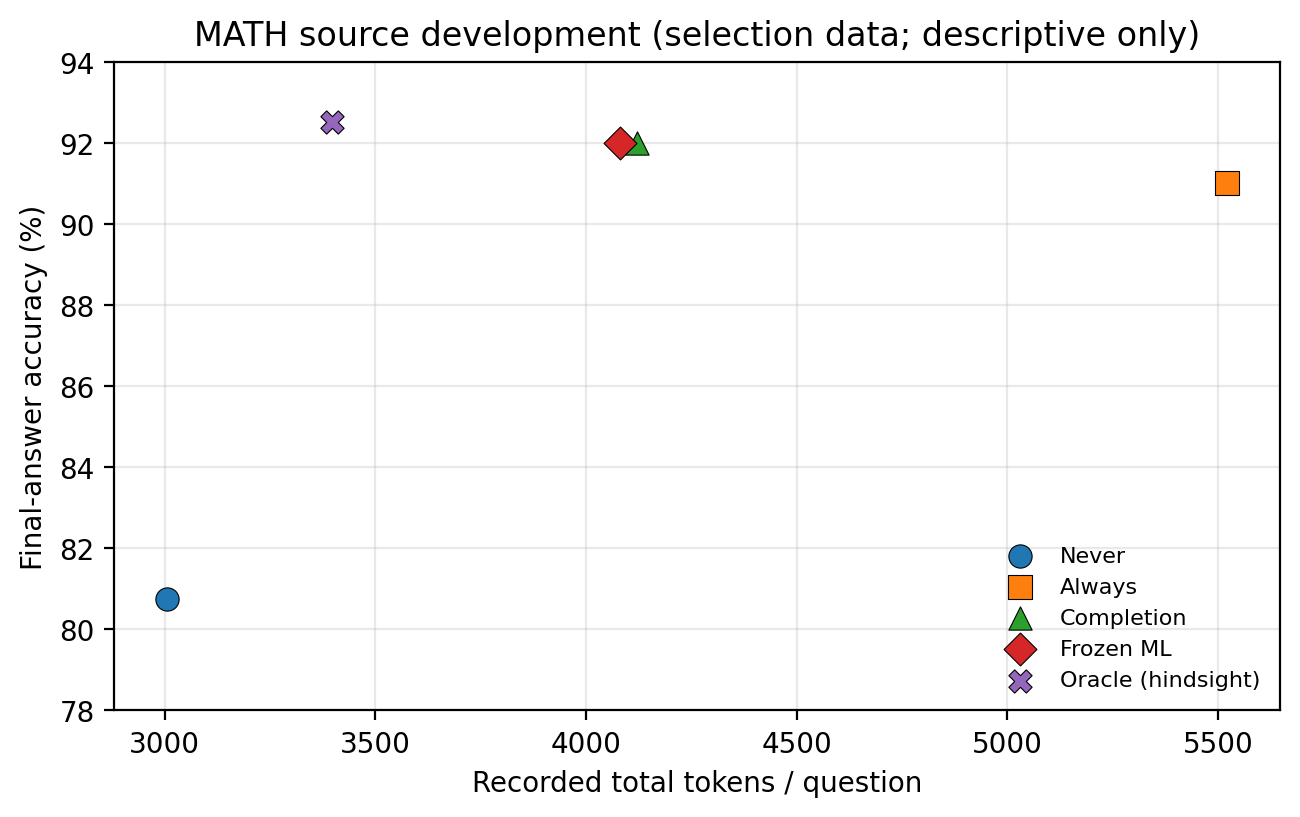
\includegraphics[width=\linewidth]{figures/source_development_accuracy_vs_tokens.png}
\caption{MATH source-development policy accuracy versus recorded token cost. This selection partition informed model/threshold selection and is shown separately from the four evaluated cohorts.}
\label{fig:development-cost}
\end{figure}

The historical source-test gate differs from completion on two rollout rows, both NO\_CHANGE; accuracy is identical while the gate uses 10.4 more tokens/question. On CSQA all 1,466 gate decisions match completion exactly. The frozen gate differs on 18 MATH500 rows across nine questions and 10 GSM8K rows across five questions; the recorded policy accuracy is lower than completion on both. The oracle's apparently better accuracy-cost point is an unattainable hindsight bound, not a feasible policy.

\begin{figure*}[t]
\centering
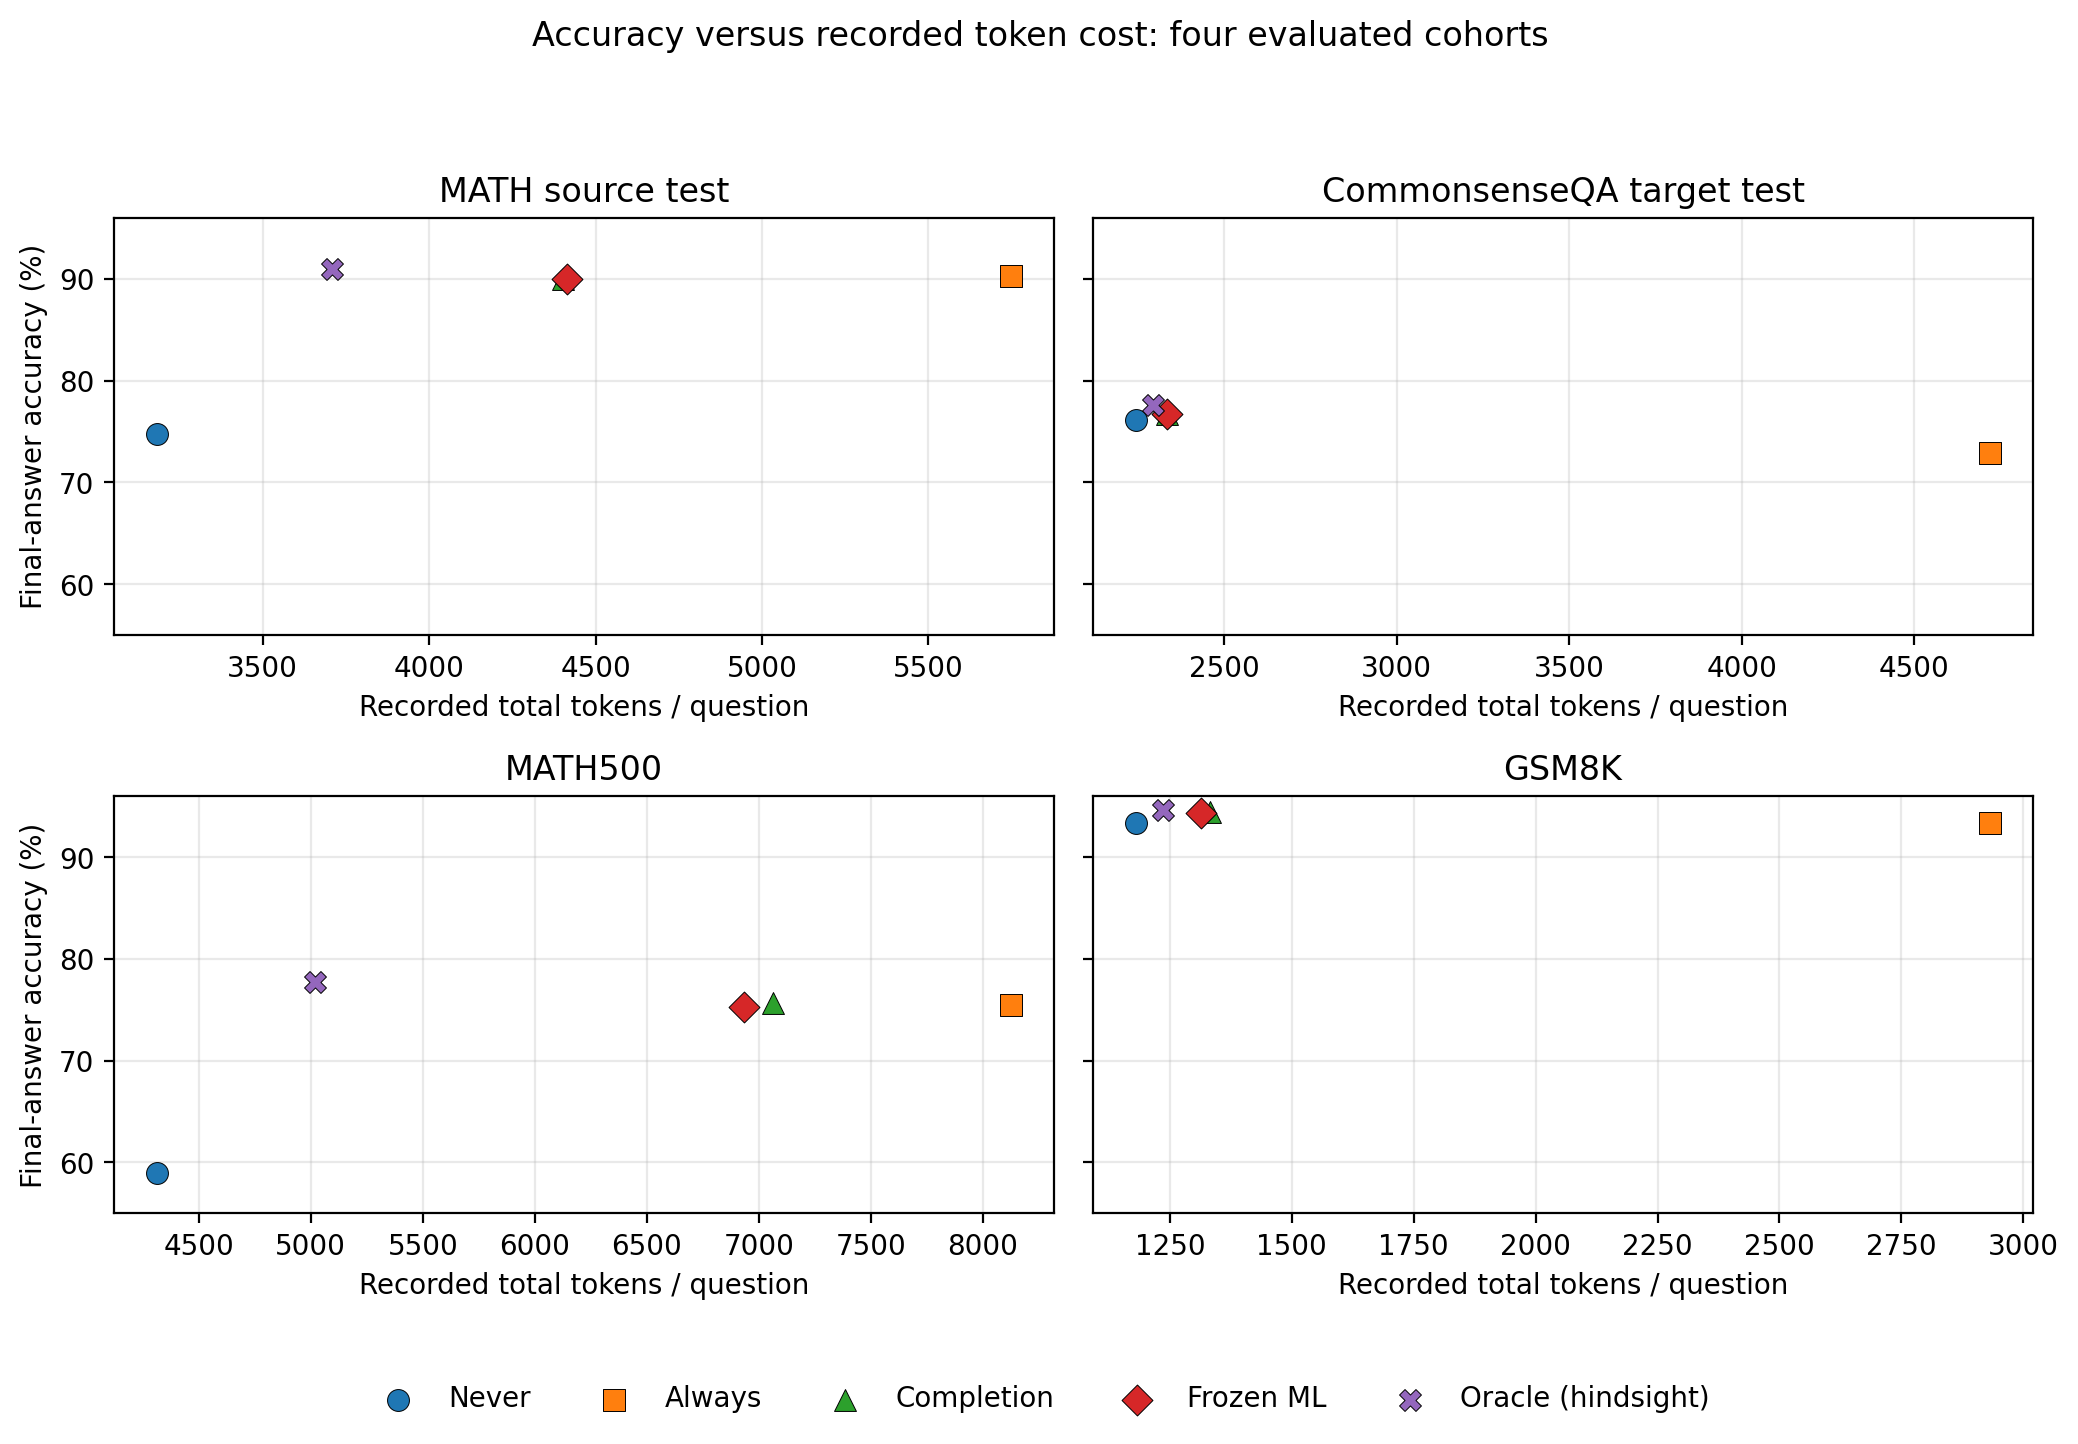
\includegraphics[width=\textwidth]{figures/accuracy_vs_tokens.png}
\caption{Final-answer accuracy versus recorded total tokens per question for the five policies in the four evaluated cohorts. The source-development partition is excluded here and plotted separately in Fig.~\ref{fig:development-cost}. Oracle points use future outcomes and are not implementable. Token use is replay accounting, not measured latency.}
\label{fig:cost}
\end{figure*}

\subsection{Paired policy differences}
Table~\ref{tab:paired} gives selected paired differences, with question-cluster bootstrap intervals. These intervals condition on saved outcomes. Sign-flip p-values are unadjusted Monte Carlo diagnostics.

\begin{table}[t]
\caption{Paired accuracy differences (percentage points) and question-cluster 95\% bootstrap intervals.}
\label{tab:paired}
\centering\scriptsize
\begin{tabular}{llrrr}
\toprule
\textbf{Cohort} & \textbf{Contrast} & \textbf{Diff.} & \textbf{95\% CI} & \textbf{$p$}\\
\midrule
MATH source test & Completion $-$ Never & 15.25 & [11.75, 18.75] & $<.0001$\\
 & Frozen ML $-$ Completion & 0.00 & [0.00, 0.00] & 1.000\\
CSQA target test & Completion $-$ Never & 0.55 & [0.14, 1.09] & .121\\
 & Frozen ML $-$ Completion & 0.00 & [0.00, 0.00] & 1.000\\
MATH500 & Completion $-$ Never & 16.70 & [13.40, 20.10] & $<.0001$\\
 & Frozen ML $-$ Completion & $-0.40$ & [$-0.90$, 0.00] & .252\\
GSM8K & Completion $-$ Never & 1.06 & [0.57, 1.59] & $<.0001$\\
 & Frozen ML $-$ Completion & $-0.11$ & [$-0.30$, 0.00] & .496\\
\bottomrule
\end{tabular}
\\[-1pt]\parbox{\linewidth}{\scriptsize Monte Carlo sign-flip tests, two-sided and unadjusted; minimum reported $p=0.00005$ shown as $<.0001$. Sparse CSQA improvements yield a positive percentile interval but an inconclusive sign-flip test ($p=.121$); do not call it significant. Nonsignificance does not imply equivalence.}
\end{table}

Completion minus never-recheck increases accuracy by 15.25 points on the source test, 16.70 points on MATH500, and 1.06 points on GSM8K. On CSQA, always-recheck reduces accuracy by 3.27 points versus never-recheck, while completion increases it by 0.55 points. The paired bootstrap interval is +0.14 to +1.09 points, but the cluster sign-flip test is inconclusive ($p=.121$) because helpful changes are sparse; this is not a significance claim. Test exposure further limits inference. The learned-minus-completion contrasts provide no evidence of an accuracy gain. Their near-zero values are not formal equivalence tests.

\subsection{Three-class classifier performance}
Table~\ref{tab:classoverall} separates argmax prediction of HELP/NO\_CHANGE/HURT from downstream policy accuracy. The classifier can have high overall accuracy while failing to identify rare classes. On CSQA, three-class accuracy is 91.54\%, but macro-F1 is 0.394; an always-NO\_CHANGE classifier would score 93.86\% because NO\_CHANGE accounts for 688 of 733 question-equivalents. The learned model's HURT recall is zero on both historical test partitions.

\begin{table*}[t]
\caption{Frozen gate classifier metrics. Supports are question-equivalent counts; raw row counts differ where repeated rollouts exist.}
\label{tab:classoverall}
\centering\small
\begin{tabular}{lrrrrrrr}
\toprule
\textbf{Cohort} & \textbf{Questions} & \textbf{HELP/NC/HURT support} & \textbf{Accuracy} & \textbf{Macro-F1 [95\% CI]} & \textbf{Weighted-F1} & \textbf{Log loss [95\% CI]}\\
\midrule
MATH source development$^a$ & 400 & 47 / 347 / 6 & 85.00\% & .559 [.494,.636] & .868 & .392 [.321,.467]\\
MATH source test & 400 & 65 / 332 / 3 & 85.25\% & .542 [.509,.572] & .869 & .411 [.334,.492]\\
CSQA target test & 733 & 10.5 / 688 / 34.5 & 91.54\% & .394 [.334,.455] & .900 & .322 [.260,.388]\\
MATH500$^b$ & 500 & 93.5 / 395.5 / 11 & 70.20\% & .465 [.432,.500] & .732 & .728 [.643,.816]\\
GSM8K$^b$ & 1,319 & 16.5 / 1,286 / 16.5 & 94.39\% & .496 [.432,.552] & .953 & .213 [.184,.243]\\
\bottomrule
\end{tabular}
\\[2pt]\parbox{\textwidth}{\scriptsize $^a$Development metrics use the partition involved in model and threshold selection. $^b$Exploratory fixed-artifact replay diagnostics, not fresh confirmation. Log loss is computed from uncalibrated saved probabilities; it should not be read as a calibration guarantee.}
\end{table*}

\begin{table*}[t]
\caption{Per-class precision, recall, and F1 for the frozen classifier. Class order is HELP, NO\_CHANGE, HURT.}
\label{tab:perclass}
\centering\small
\begin{tabular}{llrrr|llrrr}
\toprule
\textbf{Cohort} & \textbf{Class} & \textbf{P} & \textbf{R} & \textbf{F1} & \textbf{Cohort} & \textbf{Class} & \textbf{P} & \textbf{R} & \textbf{F1}\\
\midrule
MATH source test & HELP & .588 & .923 & .719 & CSQA target test & HELP & .160 & .381 & .225\\
 & NO\_CHANGE & .976 & .846 & .906 &  & NO\_CHANGE & .942 & .969 & .956\\
 & HURT & .000 & .000 & .000 &  & HURT & .000 & .000 & .000\\
MATH500 & HELP & .417 & .914 & .573 & GSM8K & HELP & .370 & .606 & .460\\
 & NO\_CHANGE & .960 & .670 & .789 &  & NO\_CHANGE & .983 & .959 & .971\\
 & HURT & .026 & .045 & .033 &  & HURT & .041 & .091 & .056\\
\bottomrule
\end{tabular}
\end{table*}

Raw confusion matrices (true rows, predicted columns; order HELP, NO\_CHANGE, HURT) are shown in Table~\ref{tab:confusion}. For the two-rollout CSQA cohort, the corresponding question-equivalent matrix is $[[4,6.5,0],[21,667,0],[0,34.5,0]]$. MATH500 and GSM8K question-equivalent matrices are half their raw counts because each question has two recorded rollouts.

\begin{table*}[t]
\caption{Raw rollout-row confusion matrices for the frozen classifier.}
\label{tab:confusion}
\centering\small
\begin{tabular}{ll}
\toprule
\textbf{Cohort} & \textbf{Confusion matrix}\\
\midrule
MATH source test & $\begin{bmatrix}60&5&0\\41&281&10\\1&2&0\end{bmatrix}$\\
CSQA target test & $\begin{bmatrix}8&13&0\\42&1334&0\\0&69&0\end{bmatrix}$\\
MATH500 & $\begin{bmatrix}171&13&3\\227&530&34\\12&9&1\end{bmatrix}$\\
GSM8K & $\begin{bmatrix}20&13&0\\34&2467&71\\0&30&3\end{bmatrix}$\\
\bottomrule
\end{tabular}
\end{table*}

\subsection{Completion state and correction events}
On source test, 62 of 65 HELP rollout rows have a length completion reason; the completion rule selects these and one HURT row. On CSQA, the rule selects 25 of 733 questions (50 of 1,466 rows), capturing 4 helpful question-equivalents and no harmful events in this recorded test; the whole cohort includes 34.5 HURT question-equivalents across two rollouts. On MATH500, length-state rows contain 179 HELP and 12 HURT events among 454 rows, whereas stop-state rows contain 8 HELP and 10 HURT among 546. On GSM8K, length-state rows contain 28 HELP and no HURT among 76 rows; stop-state rows contain 5 HELP and 33 HURT among 2,562 rows. These associations vary by task and do not show that length termination causes correctability.

The completion policy captures 95.38\% of source-test HELP outcomes, with 57.94\% helpful precision among selected rechecks. On CSQA it captures 38.10\% of HELP equivalents and helpful precision is 16.00\%. It avoids two of three source-test HURT events, all 34.5 target-test HURT equivalents, five of 11 MATH500 HURT equivalents, and all 16.5 GSM8K HURT equivalents in these records. These are finite-replay event rates, not a guarantee that the policy prevents harmful revisions on new prompts or models.

\subsection{Call Reduction Versus Token Reduction}
The completion rule selects a share of calls according to the initial completion status, but selected revisions do not have the same average token cost as skipped revisions. We independently recalculated the mean \texttt{action\_actual\_tokens} after averaging rollouts within canonical question hashes, then weighting each question equally. Table~\ref{tab:call-token-cost} reports the number of selected and skipped questions, the selected-call share, state-conditional mean revision tokens, and the share of the question-equal revision-token budget consumed by length-state rechecks. No questions had an unknown completion state in these four cohorts.

\begin{table*}[t]
\caption{Completion-selected calls and revision-token use. Call percentages count recorded intervention rows. Means first average rollouts within canonical question, then weight each question equally. Token-budget share uses question-equal per-question revision-token totals.}
\label{tab:call-token-cost}
\centering\scriptsize
\begin{tabular}{lrrrrrr}
\toprule
\textbf{Cohort} & \textbf{\shortstack{Length\\questions}} & \textbf{\shortstack{Stop\\questions}} & \textbf{\shortstack{Calls selected / all\\(\%)}} & \textbf{\shortstack{Mean action tokens\\length}} & \textbf{\shortstack{Mean action tokens\\stop}} & \textbf{\shortstack{Revision-token share\\length (\%)}}\\
\midrule
MATH source test & 107 & 293 & 107/400 (26.75) & 4,562.3 & 1,836.2 & 47.57\\
MATH500 & 227 & 273 & 454/1,000 (45.40) & 6,058.0 & 1,945.2 & 72.14\\
GSM8K & 38 & 1,281 & 76/2,638 (2.88) & 5,240.2 & 1,648.2 & 8.62\\
CSQA target test & 25 & 708 & 50/1,466 (3.41) & 2,675.2 & 2,469.4 & 3.68\\
\bottomrule
\end{tabular}
\end{table*}

The clearest divergence occurs on MATH500: the completion rule selects 45.4\% of recorded calls, yet those calls consume 72.14\% of the full revision-token budget because their mean recorded action length is much higher than that of skipped revisions. It therefore avoids 54.6\% of calls but only 27.86\% of revision tokens; after including the unchanged initial-generation cost, total replay tokens fall by 13.07\% relative to always rechecking (Table~\ref{tab:policies}). This distinction also appears in the source-test MATH and GSM8K cohorts, while the CSQA selected/skipped revision means are closer. The measurements support reporting call counts and token costs separately: fewer calls need not translate proportionally into fewer tokens. These are retrospective associations in fixed logs; completion state was not randomized, so they do not establish that length termination causes longer revisions or higher costs in a new protocol.

\subsection{Marginal Value of Learned Gating Beyond Completion}
We independently recomputed the frozen gate's actions and compared them with completion on the same recorded responses. The 30 discordant rollout rows belong to 16 canonical question groups; rollout counts therefore exceed the number of independent question units. Across these discordances, seven HELP transitions were skipped by the learned gate and no HURT transitions occurred. Table~\ref{tab:gate-marginal} reports question-equal policy differences; 95\% intervals resample canonical question groups and are conditional on this finite response library.

\begin{table*}[t]
\caption{Marginal policy effects of the frozen learned gate relative to completion. Accuracy and token differences are ML minus completion. Repeated rollouts are averaged within canonical question before question-level uncertainty estimation.}
\label{tab:gate-marginal}
\centering\scriptsize
\begin{tabular}{lrrrr}
\toprule
\textbf{Cohort} & \textbf{Disagreements} & \textbf{Accuracy (ML / completion, \%)} & \textbf{Accuracy difference, pp (95\% CI)} & \textbf{Replay-token difference/q (95\% CI)}\\
\midrule
MATH source test & 2 / 2 & 90.000 / 90.000 & 0.000 [0.000, 0.000] & +10.405 [0.000, 26.920]\\
CommonsenseQA target test & 0 / 0 & 76.6712 / 76.6712 & 0.000 [0.000, 0.000] & 0.000 [0.000, 0.000]\\
MATH500 & 18 / 9 & 75.300 / 75.700 & $-0.400$ [$-0.900$, 0.000] & $-129.228$ [$-223.461$, $-50.741$]\\
GSM8K & 10 / 5 & 94.3518 / 94.4655 & $-0.114$ [$-0.303$, 0.000] & $-18.262$ [$-37.030$, $-3.312$]\\
\bottomrule
\end{tabular}
\end{table*}

The MATH source-test gate adds two stop-completed rechecks without changing accuracy. On CommonsenseQA, all 1,466 rollout decisions agree. On MATH500 and GSM8K, the learned gate uses fewer replay tokens but has lower recorded accuracy by 0.400 and 0.114 percentage points, respectively. These differences describe an accuracy--cost trade-off in the saved records; they do not show a universal disadvantage of learned gating, nor do the intervals establish equivalence. All 28 disagreements in the two supplementary cohorts are associated with length-limited initial generations and stored finalizer answers. That finalizer record does not determine whether the event was formatting recovery, completion recovery, or a reasoning correction.

\begin{figure}[t]
\centering
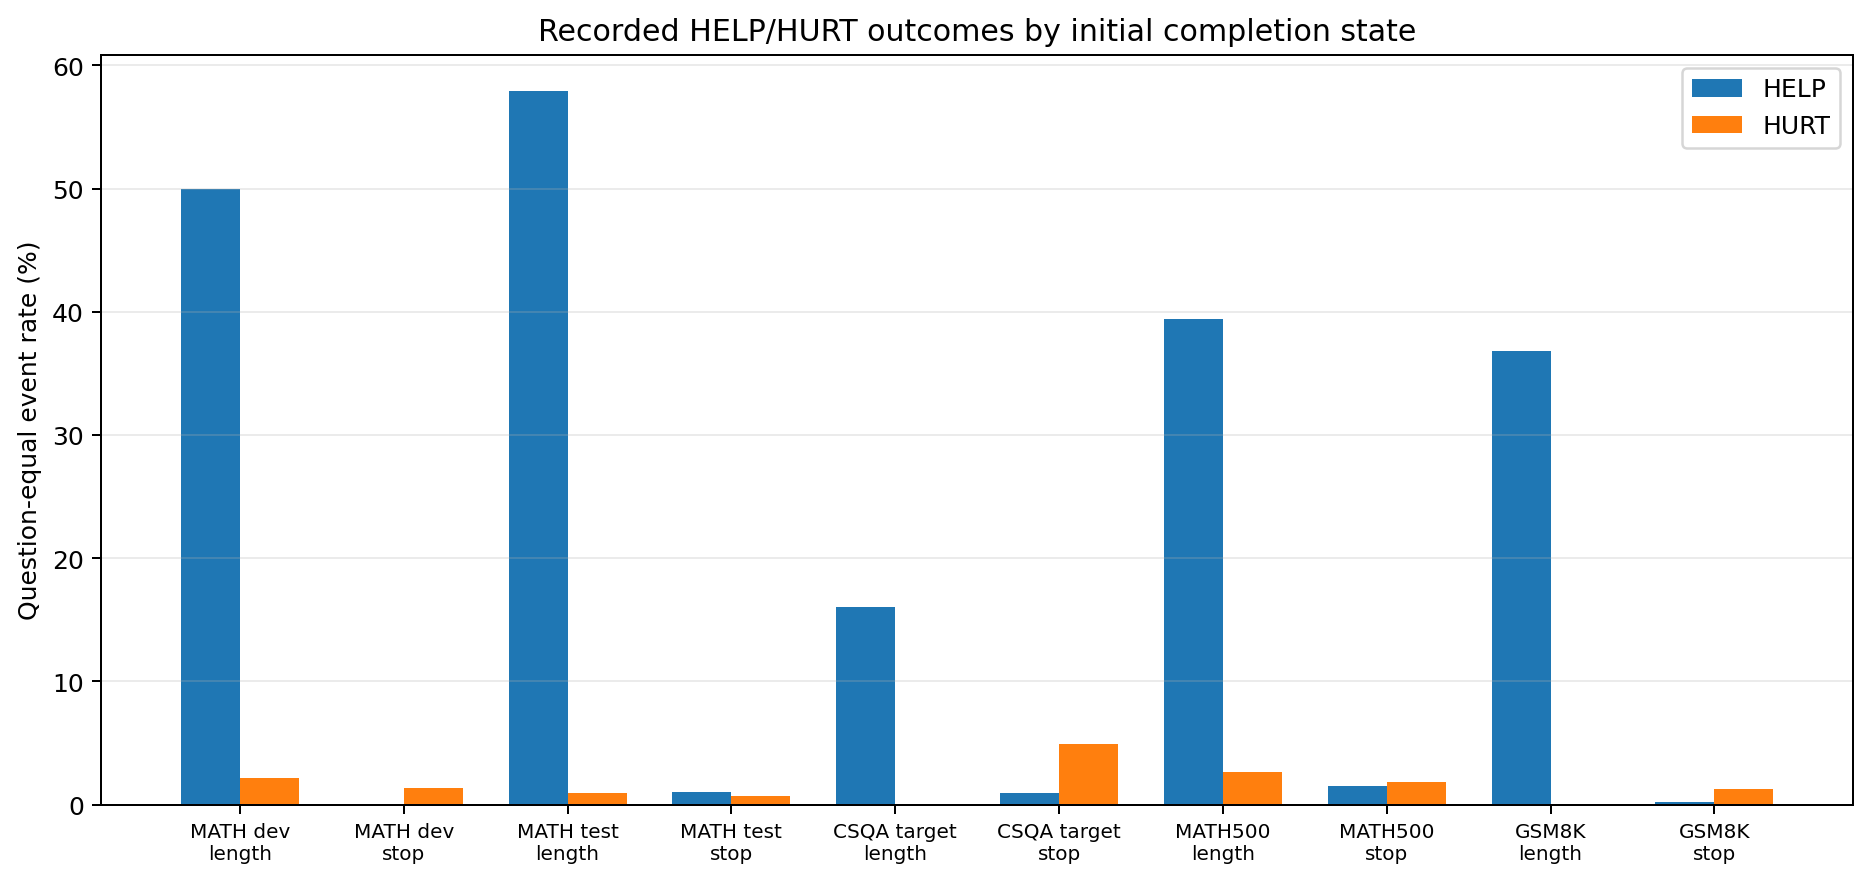
\includegraphics[width=\linewidth]{figures/help_hurt_by_completion.png}
\caption{Question-equal HELP and HURT rates by initial completion state in the recorded cohorts. Completion status is associated with different event rates across tasks; the plot is descriptive and does not imply a causal effect.}
\label{fig:completion}
\end{figure}

\section{Prospective Local Inference and Cross-Protocol Transfer}
\label{sec:local}

We conducted two separate prospective local-inference studies with Qwen3-4B-Instruct-2507 (`qwen3:4b-instruct`, Q4\_K\_M; Ollama digest \texttt{0edcdef34593eac1aa2be9c7d06c432dcf81945adca5eca2f27662c18f168ba0}). Inference ran locally with Ollama 0.40.16 on an AMD Ryzen 7 4800H, NVIDIA RTX 3050 Laptop GPU (4~GiB), and 16~GiB RAM. The frozen classifier remained the original RecheckLab v0.2 artifact with 19 initial-only features, class order HELP/NO\_CHANGE/HURT, score $p_H-p_U$, and threshold $0.25968145276947807$. It was not retrained or recalibrated. The Instruct checkpoint and prompts differ from the Qwen3-4B SEVRA recorded-response protocol, so every local gate result is a cross-model/cross-protocol OOD diagnostic.

\paragraph{Selection and answer measurement.} The GSM8K cohort contains 40 canonical-unique main/train questions, selected before inference after overlap exclusions. The hard-MATH selection froze 60 uniformly sampled eligible questions from the pinned original MATH test partition (29 Level 4, 31 Level 5; source version/revision and question hashes are preserved in the experiment manifest). Eligibility required one supported final exact integer or rational reference answer and excluded overlaps with known SEVRA/RecheckLab cohorts and prior local studies. This restriction excludes symbolic and ambiguous-answer items and may make the sample easier than the full Level 4--5 benchmark; it is not representative of all MATH questions. Source IDs, difficulty labels, and all 60 keys were independently matched to the pinned benchmark records. We reconstructed completed MATH outputs from the durable stream journal, independently extracted the final answer and compared exact rational values: all 86 completed call labels matched the saved grading labels. Six additional correct responses were checked by independent mathematical derivations; both incorrect initial responses were inspected, including the sole HELP case. The HELP response changed a parseable wrong answer to a parseable correct one, consistent with a semantic answer correction, but a single case cannot establish the model's internal reasoning mechanism. Generation prompts contained the question and protocol instructions (and the initial response for revisions); keys and correctness were stored separately. Frozen-gate decisions were recorded from initial-only fields before revisions, with no gold, correctness, or revision inputs.

\paragraph{Paired policy results.} Each policy reuses the same completed initial/revision pair. Table~\ref{tab:local-results} reports all four policies. GSM8K completed 80/80 calls with 40/40 parseable initial and revision answers; MATH completed 86 calls over 43 pairs, also with 43/43 parseable responses in both phases. Each cohort had one HELP, no HURT, and the rest NO\_CHANGE. The gate and completion rule each chose zero rechecks in both studies, so both matched never-recheck accuracy and missed the one helpful revision; always-recheck captured it. These are observed decisions on small cohorts, not evidence that the selective policies are universally equivalent or inferior.

\begin{table}[t]
\centering
\caption{Prospective local inference policy results. Replayed latency includes only the measured initial call and, when selected, the measured revision call; it excludes gate computation and is not deployed end-to-end latency.}
\label{tab:local-results}
\scriptsize
\setlength{\tabcolsep}{2.5pt}
\begin{tabularx}{\columnwidth}{llrrrr}
\toprule
Cohort & Policy & Correct & Rechecks & Tokens/q & Replay s/q \\
\midrule
GSM8K ($n=40$) & Never & 37/40 (92.5\%) & 0 & 181.3 & 5.22 \\
 & Always & 38/40 (95.0\%) & 40 & 500.2 & 10.49 \\
 & Completion & 37/40 (92.5\%) & 0 & 181.3 & 5.22 \\
 & ML gate (OOD) & 37/40 (92.5\%) & 0 & 181.3 & 5.22 \\
\midrule
MATH L4--5 ($n=43$) & Never & 41/43 (95.3\%) & 0 & 1,239.3 & 67.44 \\
 & Always & 42/43 (97.7\%) & 43 & 3,062.2 & 109.96 \\
 & Completion & 41/43 (95.3\%) & 0 & 1,239.3 & 67.44 \\
 & ML gate (OOD) & 41/43 (95.3\%) & 0 & 1,239.3 & 67.44 \\
\bottomrule
\end{tabularx}
\end{table}

\paragraph{Runtime and uncertainty.} GSM8K collection used 80 measured calls totaling 419.6 seconds (about 5.25 seconds per call). The 43 complete MATH pairs used 86 calls with a mean observed call duration of 53.7 seconds; its collection spanned about 2.85 hours, including long calls and stop/recovery intervals. Policy latency above is a replay estimate from those measured call times: it is not a trace of an online selector. Wilson 95\% intervals for the always/never accuracy estimates are 80.1--97.4\%/83.5--98.6\% on GSM8K and 84.5--98.7\%/87.9--99.6\% on MATH; paired bootstrap intervals for the always-minus-never difference include zero in both cohorts. The GSM8K difference is +2.5 percentage points (95\% paired bootstrap interval 0.0 to +7.5); MATH is +2.3 points (interval -7.0 to 0.0). These intervals are descriptive and do not establish significance, equivalence, or generalization.

\paragraph{Early stopping and transfer interpretation.} The MATH selection remained 60 questions, but the study was stopped after 43 complete pairs: 47 selected questions were attempted, four initial calls remained incomplete, no revision call was incomplete, and 13 questions were unattempted. Q1's inherited incomplete attempt was preserved and not retried. The primary paired comparison uses only complete pairs; longer-running or otherwise incomplete items may differ in difficulty, response length, or extraction behavior, so the 43 are not a random sample of the frozen 60. The observed zero-recheck behavior means the learned and completion gates were inactive under these Instruct protocols. It does not establish that either policy would remain inactive under other prompts, models, or completion distributions. In contrast, historical SEVRA replays include cohorts in which completion and learned decisions did select revisions; those recorded-response results are not directly comparable to these local outcomes. SEVRA itself studies selective verification with its own solver, action protocol, and gates~\cite{dip2026sevra}; the present cross-protocol diagnostic is not deployment validation and does not reproduce SEVRA's method or claims.

\section{Discussion}
\subsection{Why completion matches the learned gate}
The most direct interpretation of the recorded comparisons is that much of the useful selection signal is already represented by initial completion status. In the MATH source test, completion captures 62 of 65 HELP rows and the learned gate selects almost the same cases, while adding two NO\_CHANGE decisions. On CSQA the two policies select exactly the same rows. In the additional replays they disagree on relatively few question clusters, and those differences do not improve the gate's recorded accuracy. A prior source-training feasibility analysis found only six completed/nonempty beneficial switches and a nested-OOF residual-score AUC of 0.449; this is exploratory evidence with very few positive events, not proof that no initial-state feature can ever help.

The separate disagreement audit quantifies this marginal value: 30 rollout disagreements represented 16 question groups, with seven skipped HELP transitions and no HURT transitions. Five groups had a negative ML-minus-completion accuracy effect and 11 were neutral; none favored ML on accuracy. The gate's lower replay-token use on MATH500 and GSM8K comes from skipping length-selected revisions, most of whose disagreement rows were NO\_CHANGE, while also missing some recorded helpful revisions. Conversely, the two MATH source-test gate-only actions were neutral and added cost, and CSQA had no action disagreement. Redacted case studies show that these mechanical patterns include both a stop-completed correct answer receiving a neutral extra recheck and length/finalizer records with HELP or mixed rollout outcomes. A disagreement is therefore not itself evidence of a particular reasoning failure.

Class imbalance also matters. NO\_CHANGE accounts for 83.0\% of MATH source-test outcomes and 93.86\% of CSQA question-equivalent support. The CSQA gate's 91.54\% three-class accuracy is below the trivial NO\_CHANGE classifier's 93.86\%, while HURT recall remains zero. Thus, overall classification accuracy is not evidence of reliable revision-risk detection. The policy threshold is not argmax classification: it uses $p_H-p_U$, so policy HELP capture and multiclass HELP recall are distinct quantities.

\subsection{Domain variation and cost interpretation}
The same fixed gate and completion rule behave differently across the released cohorts. MATH500 has comparatively frequent length outcomes and a 45.4\% completion recheck rate; GSM8K has only a 2.88\% completion recheck rate. CSQA's completion rule selects 3.41\% of question-equivalent outcomes, while always-recheck lowers final accuracy versus never-recheck. These contrasts are consistent with task-level heterogeneity in the saved outcomes, but they do not isolate a causal domain effect: benchmark composition, prompts, answer extraction, and inherited response protocol may differ.

Recorded token savings are largest for highly selective policies, but costs are reconstructed from saved prompt-plus-generation token counts. No trustworthy per-call wall-time observations were available in the project timing audit. We therefore make no latency, energy, memory, or monetary-savings claim. Classifier inference overhead was not measured as a live serving comparison.

\subsection{Contribution relative to SEVRA}
SEVRA is the response-generation and selective-verification antecedent, including the source of the paired outcomes. The present analysis contributes a separate frozen RecheckLab artifact and an explicit comparison with a completion baseline across existing released response logs. The empirical conclusion is negative for the learned gate: it does not demonstrate incremental accuracy over completion. This is a reproducible secondary evaluation, not a new selective-verification algorithm or independent benchmark collection. The breadth of available evidence does not support a claim that the classifier generalizes to unseen prompts, checkpoints, or an independently collected deployment environment.

\section{Threats to Validity}
\subsection{Data provenance and outcome validity}
The v0.2 labels and intervention responses were inherited from SEVRA. Its public data card says gold answers were used to create outcomes but are omitted from the release. We did not independently verify each gold answer, parse, or upstream grader. Final-answer correctness consequently cannot be interpreted as an adjudicated measure of reasoning quality. For the historical records, exact checkpoint identity and full prompts remain unavailable. The local Instruct studies preserve an exact checkpoint digest and prompts but intentionally differ from the historical protocol; the frozen gate results there are OOD diagnostics.

\subsection{Benchmark and exposure limitations}
The MATH source development/test partitions are drawn from the SEVRA MATH-training release. They are not official MATH Level 5 test results. MATH500 is a separate released evaluation split. Source test, CSQA target test, MATH500, and GSM8K have all been inspected in prior project work; our reanalysis and frozen-gate scoring cannot be presented as fresh untouched confirmation. Canonical query hashing found no overlap among the included cohorts, but this does not assess model pretraining contamination.

\subsection{Statistical uncertainty and repeated rollouts}
Question clustering avoids treating repeated response rollouts as independent questions, but most external cohorts have only two recorded intervention rollouts per question. Cluster bootstrap uncertainty is conditional on these finite records and underestimates uncertainty about unobserved model stochasticity or protocol changes. Harmful events can be rare; zero observed HURT selected in a cohort is not proof of zero harm risk. Many policy/cohort contrasts were examined and sign-flip p-values are unadjusted. The analysis is descriptive and was not preregistered.

The gate-versus-completion disagreement intervals likewise resample canonical questions, not rollout rows, and are conditional on inherited outcomes. In MATH500 and GSM8K, the 28 discordant records have length-limited status and a stored finalizer-produced answer, but the logs do not expose enough provenance to decide whether finalization recovered an answer, changed formatting, or repaired reasoning. The parsed-answer and correctness-transition fields cannot establish semantic reasoning quality; we did not adjudicate these cases against gold answers or revise any inherited labels. These additional retrospective contrasts are exploratory and do not provide a fresh independent evaluation.

\subsection{Selection, distribution, and policy scope}
Source development informed model and threshold selection, so its policy metrics are descriptive and optimistic for selection. The frozen artifact was not adapted on target data in this study. Only one model family, one recorded active-verification action, and a limited set of task cohorts are represented. Completion-state associations are not causal. A different initial budget, prompt, finalizer, model checkpoint, or action could alter both the base error rate and the value of rechecking.

\subsection{Efficiency measurement}
Token totals represent saved replay fields; they do not establish wall-clock latency, throughput, GPU utilization, energy, or monetary cost. Always-recheck token totals combine base and intervention records, while the selective policy uses a counterfactual mask over the same recorded intervention costs. This is an accounting estimate of what those fixed outcomes would cost under each policy, not a measured serving trace.

\section{Conclusion}
The evidence spans historical SEVRA recorded-response replay, exploratory SEVRA MATH500/GSM8K replay, and two prospective local-inference cohorts on GSM8K and a selected exact-answer MATH Level 4--5 subset. Historical replay shows no demonstrated incremental accuracy for the frozen RecheckLab gate over completion. In the local Instruct cohorts, both the completion rule and the frozen gate selected zero rechecks and therefore matched never-recheck accuracy, while always-recheck captured the single HELP in each small study. The MATH study stopped with 43 complete pairs from a frozen 60-question selection, and its exact-answer restrictions and runtime censoring limit interpretation. Local gate scores are cross-model/cross-protocol OOD diagnostics, not deployment validation; the observed inactive policies do not establish universal equality or inferiority, nor do HELP labels alone establish a reasoning mechanism. The available evidence supports further prospective evaluation with broader answer types, completed and adequately powered samples, and measured end-to-end serving costs; it does not establish a general accuracy or latency advantage for learned gating.

\bibliographystyle{IEEEtran}
\balance
\bibliography{references}
\end{document}
